\documentclass[
  11pt, % 10pt - 12pt
  %letterpaper
  %indonesian
]{assignment}

% Template-specific packages
\usepackage{mathpazo} % Use the Palatino font

\usepackage{graphicx} % Required for including images
\usepackage{booktabs} % Required for better horizontal rules in tables

\usepackage{amsmath} % Math!
\usepackage{amssymb} % Math symbols!
\usepackage{listings} % Required for insertion of code
\usepackage{enumerate} % To modify the enumerate environment

% https://castel.dev/post/lecture-notes-2/#including-inkscape-figures-in-a-latex-document
\usepackage{import}
\usepackage{xifthen}
\usepackage{pdfpages}
\usepackage{transparent}

\newcommand{\incfig}[1]{%
    \def\svgwidth{\columnwidth}
    \import{./graphics/}{#1.pdf_tex}
}

\newcommand{\ipAddress}[1]{{\fontfamily{cmtt}\selectfont #1}} % IP Address custom style!

% ! CUSTOM - LST Preset
\lstset{
    language=SQL,
    frame=single, % Frames
    showstringspaces=false, % Don't put marks in string spaces
    numbers=left, % Line numbers on left
    numberstyle=\tiny, % Line numbers styling
    breaklines,
    basicstyle=\fontfamily{cmtt}\selectfont\small,
    columns=fullflexible,
}


%----------------------------------------------------------------------------------------
%	ASSIGNMENT INFORMATION
%----------------------------------------------------------------------------------------

% Student name
\author{Christopher Angelo - 2440041503}
% Institute or school name
\institute{BINUS University\\ Global Class}


% Due date
\date{Apr 25th, 2022}
% Assignment title
\title{Mid-Semester Exam Answer}

% Course details
\class{Software Engineering (COMP6640001)}
\professor{Ms.\ Zulfany Erlisa Rasjid}

%----------------------------------------------------------------------------------------

\begin{document}
\maketitle

%----------------------------------------------------------------------------------------
%	ASSIGNMENT CONTENT
%----------------------------------------------------------------------------------------

\section*{Question Statement}
\begin{problem}
Traffic Control division in the Police Department are having problems in monitoring traffic violation. Currently all traffic violations must be observed by the police on site. And then the officer in charge will give violation tickets on the spot. The problem with this method is that several violations can be missed, for example if the officer is writing the violation, some offender might go unnoticed. As a Software Engineer, you want to provide solution for this.

\medskip

The following are some basic requirements for this system:
\begin{itemize}
  \item CCTV will be used in an intersection. With heavy traffic. Low traffic is not considered because the officer in charge should have no problem identifying.
  \item Speed sensors will be used in roads or tollway that has speed limits. The speed sensors will be able to create a snapshot of the speeding car.
  \item Assuming the CCTV and Sensors are connected to some system that allows you to get violation information such as: license plate number, type of violation (date, time, CCTV ID or Sensor ID, speeding, traffic lights, accidents)
  \item Your application is to monitor the incidents based on the data obtained by the CCTV/Speed Sensors.
  \item The officer in the monitoring room will direct the violation to the appropriate police division.
  \item Once handled in the division, a status will be confirmed (not completed, in progress or completed)
  \item The police division head will need to see the report violation weekly and attend to those that has not been handled.
  \item The DMV (Department of Motor Vehicle) can be connected to your system, as the DMV System have all the list of license plate and its owner.
  \item Violation received by Officer on site must be input into the system by a data entry clerk.
\end{itemize}
\end{problem}

\pagebreak

\section*{Question 1}

\begin{problem}
\begin{enumerate}[a.]
  \item To choose the correct process model, compare and contrast 3 process models of your choice that you think is appropriate for this case
  \item Choose the model for this system based on the analysis performed in question 1a. and provide your reasons
\end{enumerate}
\end{problem}

\subsection*{Answer 1a}

There are a couple of process models that can be used for this system:

\subsubsection*{Waterfall Model}

The Waterfall Model is the oldest and the simplest process model. It contains 5 steps: communication, planning, modeling, construction and deployment. By the nature of the steps, one can't go back to the previous steps to change something along the line, therefore making the program faster to develop as everyone should know what they're doing. Though, it is a double-edged sword as a mistake or a change could ruin the whole system.

\subsubsection*{Incremental Model}

The Incremental model adapts the Waterfall model and make it such that one will break the large task into smaller tasks. These smaller tasks will then be developed using the Waterfall model incrementally, sometimes almost in parallel. This model is suitable for a never ending process, such as a system that needs to be developed incrementally. It is somewhat slower compared to other models but it provides a sustainable environment for development.

\subsubsection*{Agile Model}

Nowadays, the Agile Development model is one of the most popular model for software development. The aim is to provide rapid and adaptive response to changes by including customers and stakeholders into the development process. When a change is wanted, this model allows it to be done in a quick and efficient way, reducing time and cost.

\subsection*{Answer 1b}

From the analysis above, I will be choosing the \textbf{Waterfall Model}. This is due to the nature of the project (goverment project) and the fact that the project alone is not too big. There is a theoretical `final' state of the app in which after that, there will be no more changes.

\section*{Question 2}
\begin{problem}
\begin{enumerate}[a.]
  \item Identify the stakeholder for this system
  \item Write down the requirement and assumptions from the appropriate stakeholder, adding other requirements (minimum 2 other requirements and 2 assumptions) that are not listed in the case.
  \item Create a scenario-based model for this system
  \item Create a behavioral model for the violation (state diagram).
\end{enumerate}
\end{problem}

\subsection*{Answer 2a}

In this case, the stakeholders of this system are the police department (specifically officers) and the DMV.

\subsection*{Answer 2b}

The following is the requirements and assumption from stakeholders:

\textbf{Police department}

Requirements:
\begin{itemize}
  \item Integrates camera and speed sensors to get violation information
  \item Captures snapshot of the speeding car along with their speed and compiles it to a report
  \item Able to handle manual incident inputs
  \item Able to handle and store backlogs of incidents
  \item Provides a report on how incidents pans out over time
\end{itemize}

Assumptions:
\begin{itemize}
  \item Able to monitor and capture data on the streets, 24/7, both in the dark and in the light, with different road conditions (fog, extreme heat, etc).
  \item Will handle emergency incidents (emergency vehicles bypass, car crashes, etc) properly.
\end{itemize}

\bigskip

\textbf{DMV}

Requirements:
\begin{itemize}
  \item Use the provided DMV API / messaging queue safely and securely with idempotent requests.
  \item Will not need a major rework of the pre-existing DMV system.
\end{itemize}

Assumptions:
\begin{itemize}
  \item Does not process unneeded data.
  \item Does not abuse the DMV system and falsely flag violations.
\end{itemize}

\pagebreak

\subsection*{Answer 2c}

The following is the scenario-based model represented via an activity diagram for this system

\begin{figure}[h!]
  \centering
  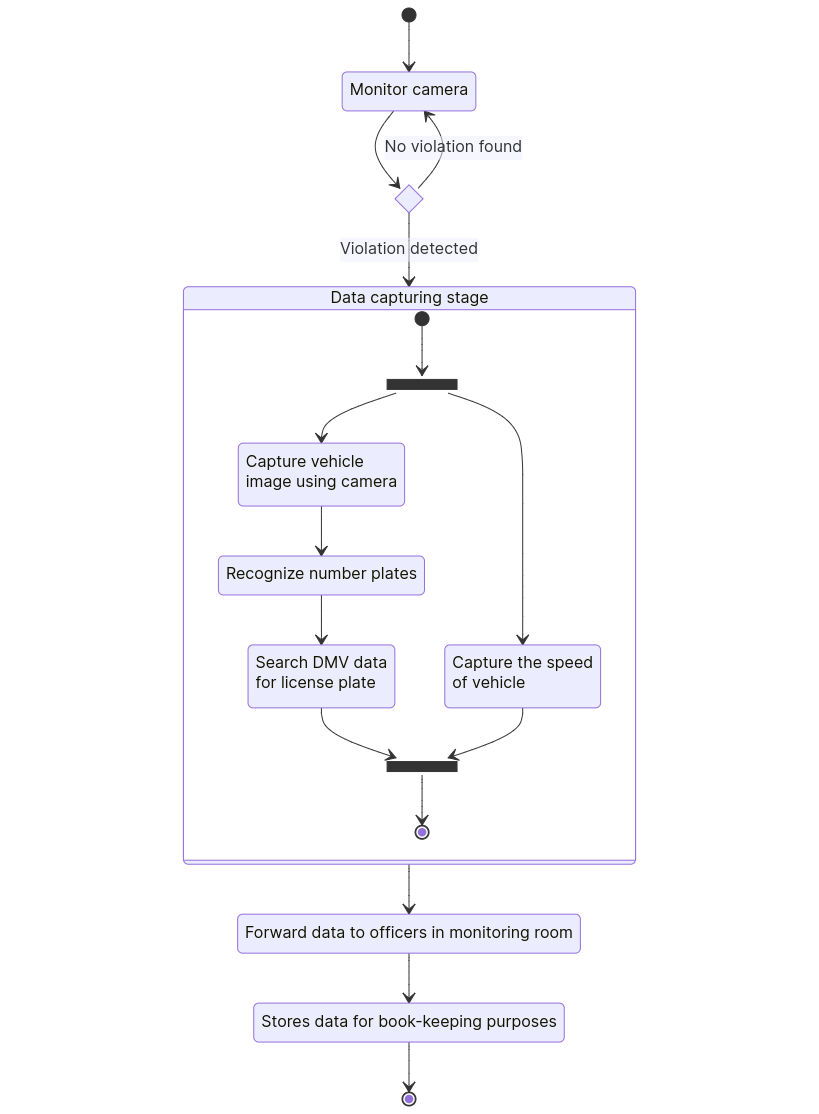
\includegraphics[width=\linewidth]{graphics/activity.png}
  \caption{A high-level activity diagram for the system}
\end{figure}

\pagebreak

\subsection*{Answer 2d}

The following is the state diagram of how the system would work.

\begin{figure}[h!]
  \centering
  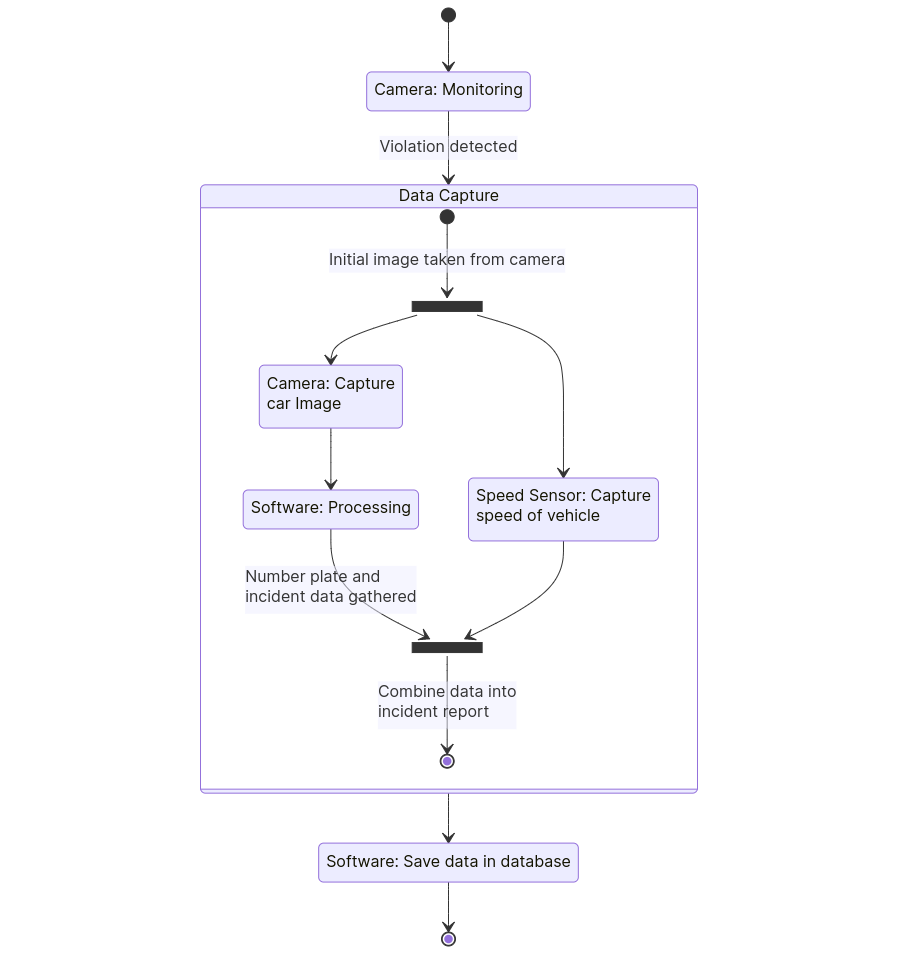
\includegraphics[width=\linewidth]{graphics/state.png}
  \caption{A high-level state diagram of the system}
\end{figure}

\pagebreak
% ---------------------------------------

\section*{Question 3}
\begin{problem}
\begin{enumerate}[a.]
  \item How is the concept of coupling related to quality of your design?
  \item Construct the component-Level diagram for this system
  \item Construct a deployment diagram for this system
\end{enumerate}
\end{problem}

\subsection*{Answer 3a}

Coupling is the degree of how `free' modules of a component are. Level of coupling generally needs to be balanced between cohesion such that components are low / weakly coupled while it is highly cohesed.

In the context of this system, modules are independence of each others. As seen in Figure~\ref{fig:component}, Coupling between components are minimized as auxiliary component (Camera, SpeedSensor, etc) have as little connection as possible (Most-likely only 1).

\subsection*{Answer 3b}

The following is the component diagram for this system

\begin{figure}[h]
  \centering
  \def\svgwidth{\columnwidth}
  \fontsize{6}{15}\selectfont
  \import{./graphics/}{ComponentDiagram.pdf_tex}
  \caption{High-Level Component Diagram}
  \label{fig:component}
\end{figure}

\pagebreak

\subsection*{Answer 3c}

The following is a deployment diagram for this system

\begin{figure*}[h]
  \centering
  \def\svgwidth{\columnwidth}
  \fontsize{9}{15}\selectfont
  \import{./graphics/}{Deployment Diagram.pdf_tex}
  \caption{Deployment Diagram}
\end{figure*}

% ---------------------------------------

\section*{Question 4}
\begin{problem}
\begin{enumerate}[a.]
  \item What qualities are expected in the:
        \begin{enumerate}[i.]
          \item Requirement
          \item Design
          \item Codes
        \end{enumerate}
  \item Explain steps on how to measure the availability of your software, by using an example
\end{enumerate}
\end{problem}

\subsection*{Answer 4a}

\subsubsection*{Requirement}

All stakeholders should have a clear understandings on what they expect out of the program. The said understanding should be exclaimed to the designers and developer in clear terms.

\subsubsection*{Design}

Design should be abstracted properly, adapted to the requirements, and should be able to be easily changed. It should consider a modular designs but with a medium-sized modules.

\subsubsection*{Code}

Code is tested using unit tests. A linter is used to ensure that the code is clean and free of common pitfalls. A shared editor config is used to ensure that the code style is consistent among programmers and IDEs\@. A pre-commit / pre-push hook is used to automatically run these checks before the code is pushed.

\subsection*{Answer 4b}

Our software's availability can be measured by monitoring the uptime of the system. The measurement can be further extended by introducing a constant health check that checks for internal system functions.

An example health check function may check for the following:
\begin{itemize}
  \item Processing unit temperature
  \item Storage health and capacity
  \item Connection status to DMV
  \item Whether all endpoints are reachable
\end{itemize}

The health check will fail if any of the above conditions is not met. If the health check fails, the system can notify people responsible for it (pager duty).

\section*{Question 5}
\begin{problem}
\begin{enumerate}[a.]
  \item Describe 5 different software testing strategies.
  \item With regards to this system, describe your strategies to test the software. Make sure that you wanted to deliver a good quality software. You should at least use 3 different strategies and explain why you would want to use these strategies.
\end{enumerate}
\end{problem}

\subsection*{Answer 5a}

\begin{itemize}
  \item Unit Testing - The smallest scope of test for a system. This test is designed to test the functionality of a single module, more specifically on how functions behave when given different inputs.
  \item Integration Testing - The scope of test for a system is larger than unit testing. This test is designed to test the functionality of a system when combined with other modules / component. For example, this test relieves when using a different version of database which might break some part of the functionality.
  \item Validation Testing - Validation testing is a test which checks whether the system has been fully functional to the specification uphold by stakeholders. This test is majority done manually also by the stakeholders.
  \item System Testing - This test whether the designed software should work with systems with different environment (i.e, software version and variant, operating system, etc).
  \item Higher Order / Usability Testing - This is the ultimate test whether the software is usable by the end user. This test shouldn't fail if everything is designed properly.
\end{itemize}

\subsection*{Answer 5b}

If I asked, for this system specifically, I am going to use \textbf{unit-test}, \textbf{integration-test} and an optional \textbf{system-test} for the testing workflow.

\medskip

Unit-tests helps when you are trying to figure out how your code works. They are the simplest and most straightforward way are the most reliable way to test one's code. This also helps with unionizing code with the expected architechture.

\medskip

When combining various external components / services, integration test is needed to ensure compatibility between components and the actual system.

\medskip

When deployed using an containers (Docker / Kubernetes) instead of virtual machines (VMWare, Virtual Box, etc), they ensure that all machine will have the same environment as it essentially `isolates' the app from the environment. This essentially solves the `it works on my machine but not on production' problem.

\end{document}
